\chapter{L'intelligenza}
La fase di costruzione dell'intelligenza che dovrebbe permettere di comprendere quando vengono suonate le note in una traccia audio si è divisa in due fasi. La prima è stata quella di riconoscere la differenza tra nota e non nota dati dei audio selezionati manualmente senza considerare la lunghezza. In un secondo momento si è poi proceduto dividendo i campioni di note in più parti di uguale lunghezza, associando a ogni divisione del campione un valore che va da 1 a 5, ovvero delle classi che indicano, essere certamente una nota associandovi la classe 5, o essere certamente non una nota accoppiando il campione alla classe 1.\\
Le tracce di strumenti fornitemi dal tutore e utilizzate per gli esperimenti sono state quelle di: 
\begin{itemize}
	\item Contrabbasso
	\item Spazzolata di rullante
	\item Colpo di rullante
	\item Colpo di cassa
\end{itemize}


\section{Prima fase}
In questa fase lo scopo è stato appunto comprendere se una macchina con le features selezionate è in grado di riconoscere la differenza tra nota e non nota. Una volta creato il file arff contenente le informazioni necessarie tramite un apposito script python lo stesso file è stato usato per costruire l'albero decisionale utilizzando l'algoritmo J48 (versione più fine di ID3 descritto nel Capitolo 2) ottenendo come risultato le matrici di confusione\footnote{Le colonne di queste matrici di confusione indicano il valore atteso, sulle righe vi sono invece i valori risultanti} per gli strumenti sopra elencati in figura \ref{fig:cm_1}\\

I campioni da classificare erano divisi in due classi: ``si'' e ``no'' identificanti note e non note. Nella tabella \ref{tab:numerosità_1} si può osservare la numerosità di campioni per ogni classe, la classe con meno campioni è quella del colpo di rullante vista la natura delle tracce audio, è stato complesso estrarre dei campioni adatti vista la natura dello strumento e della registrazione, infatti le note erano spesso molto vicini tra loro e confusi oltre che essere molto inferiori rispetto a quelle degli altri strumenti.

\begin{table}[h!]
	\begin{center}
		\begin{tabular}{l|c|r} % <-- Alignments: 1st column left, 2nd middle and 3rd right, with vertical lines in between
			\textbf{Classe} & \textbf{Si} & \textbf{No}\\
			%			$\alpha$ & $\beta$ & $\gamma$ \\
			\hline
			Basso & 121 & 94\\
			Spazzolata di Rullante & 80 & 73\\
			Colpo di Rullante & 64 & 73\\
			Cassa & 132 & 72
		\end{tabular}
		\caption{Numerosità campioni prima fase.}
		\label{tab:numerosità_1}
	\end{center}
\end{table}

\begin{figure}[h!]
	\centering
	\begin{subfigure}{.5\linewidth}
		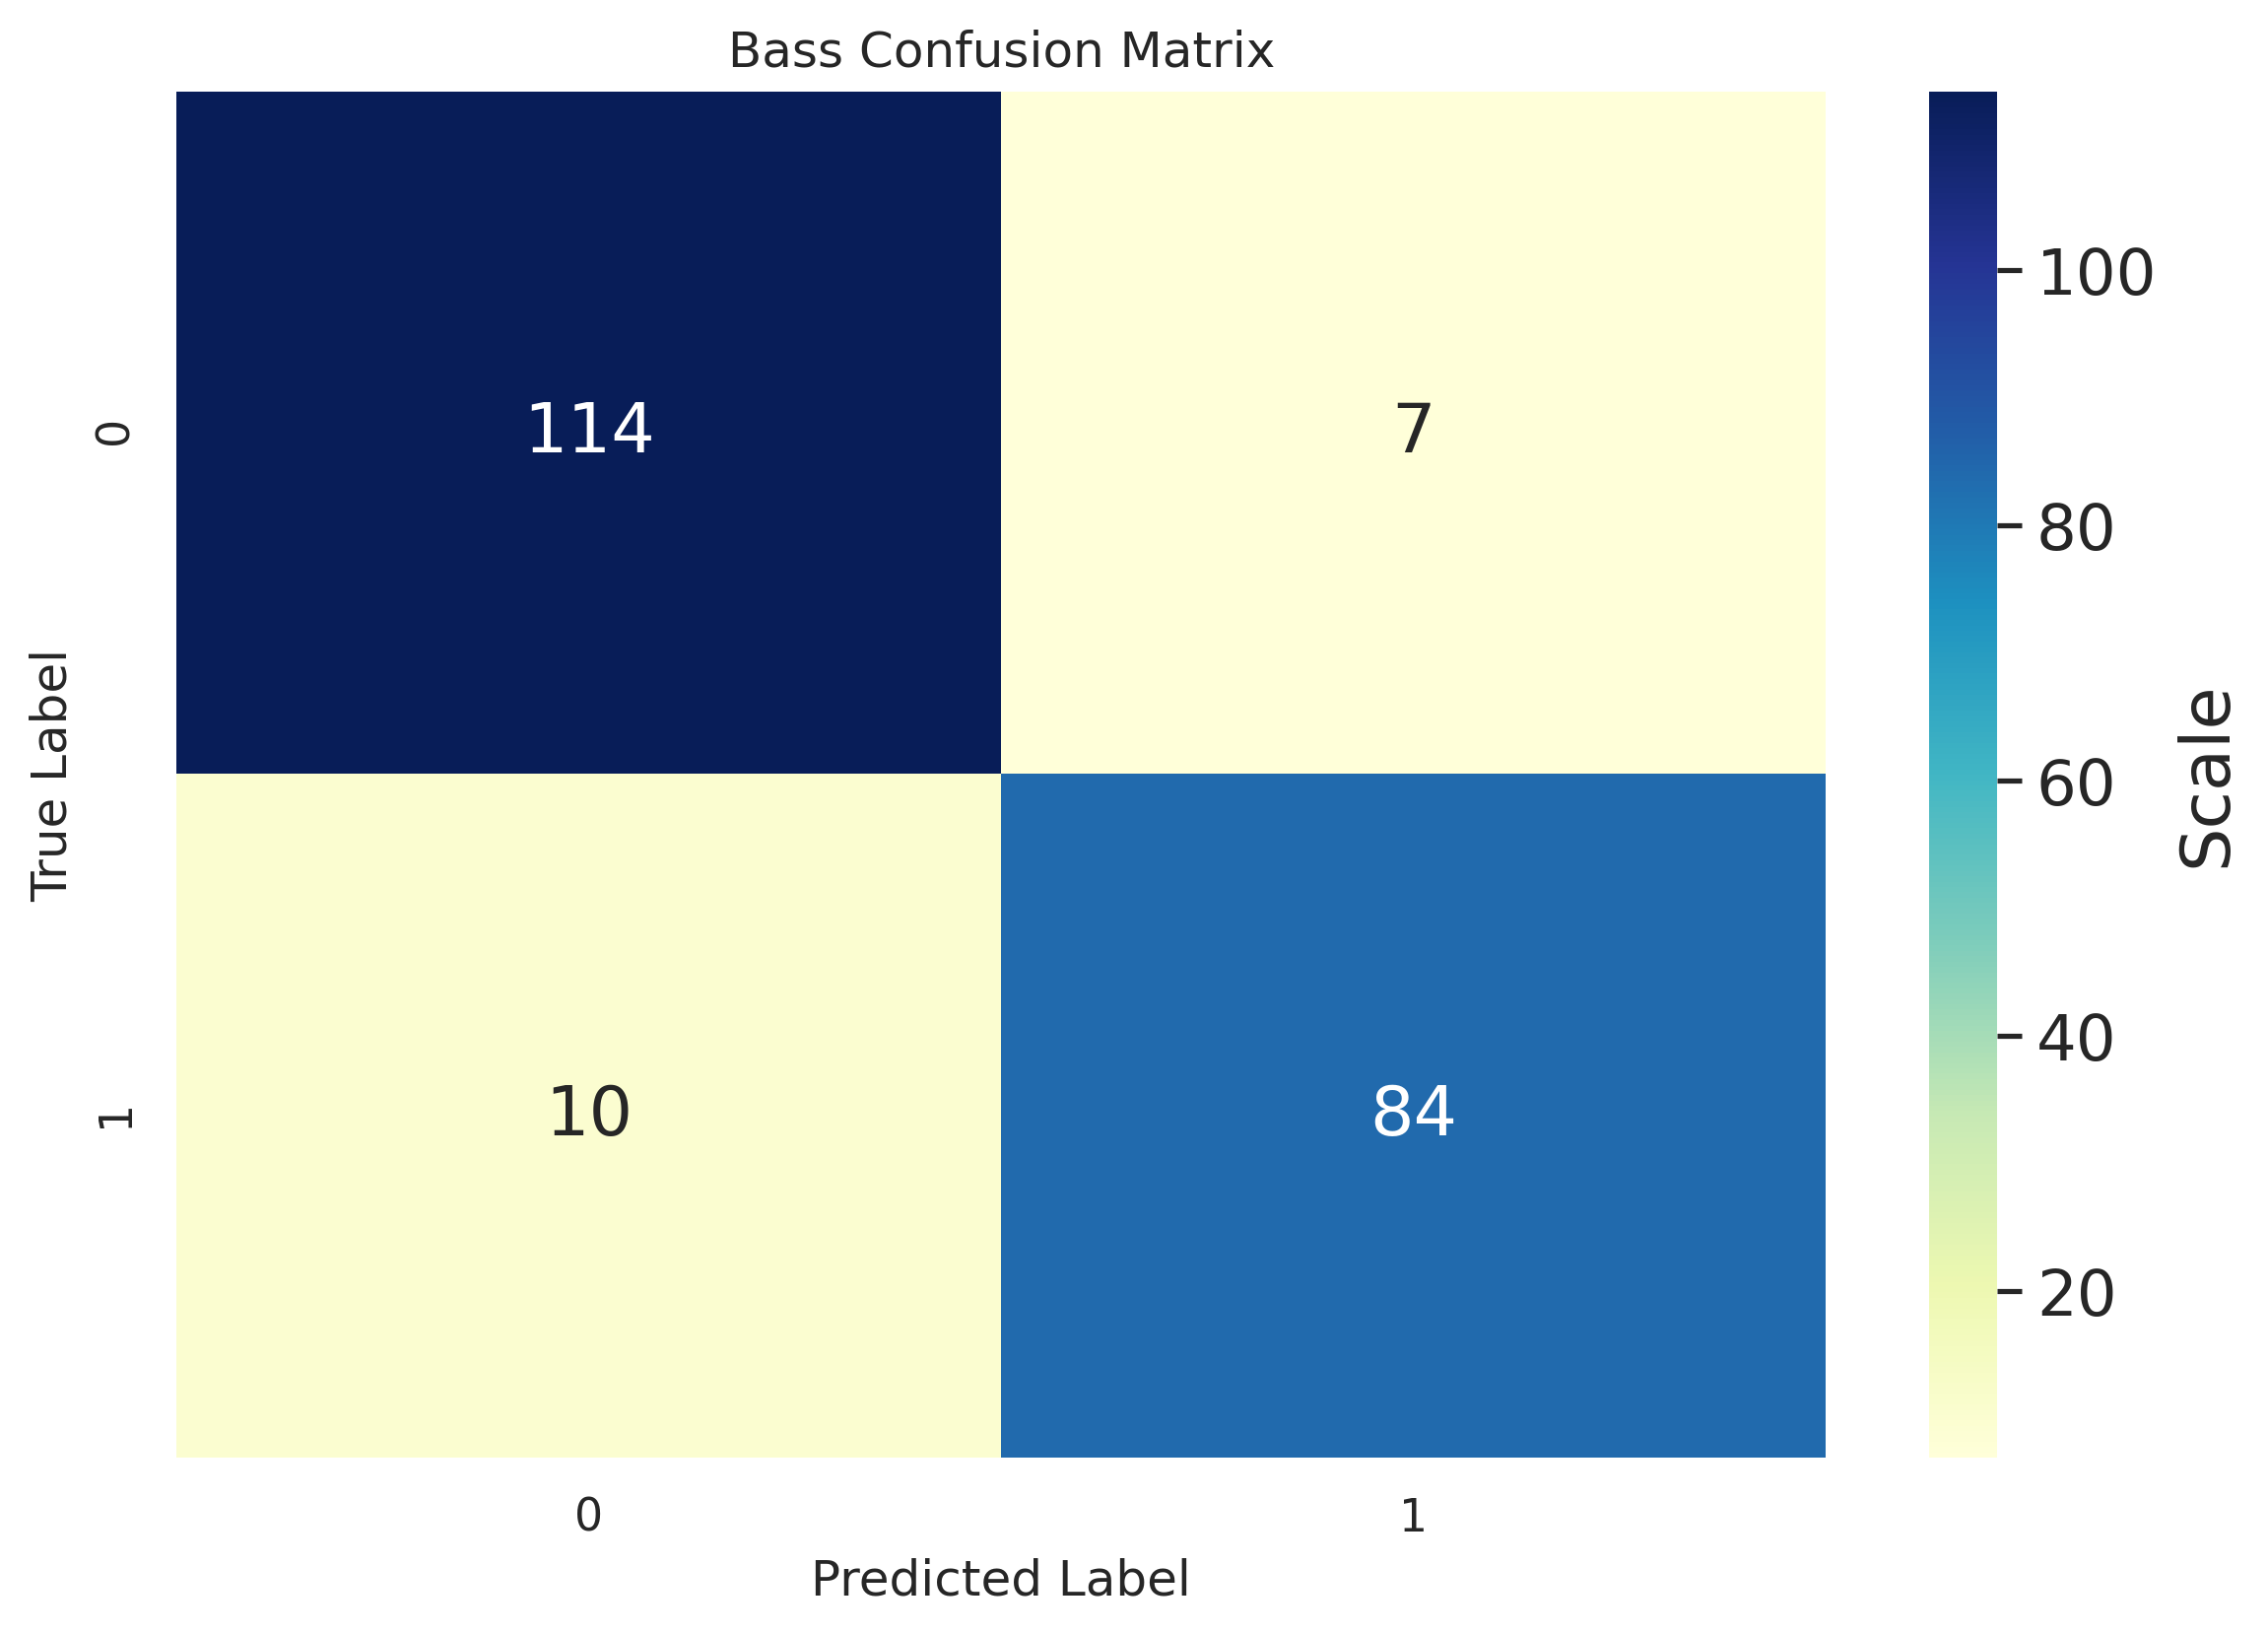
\includegraphics[width=\linewidth]{./immagini/first_classification/cb_cm.png} 
		\caption{Matrice di confusione per il basso}
		\label{fig:cm_1a}
	\end{subfigure}\hfill
	\begin{subfigure}{.5\linewidth}
		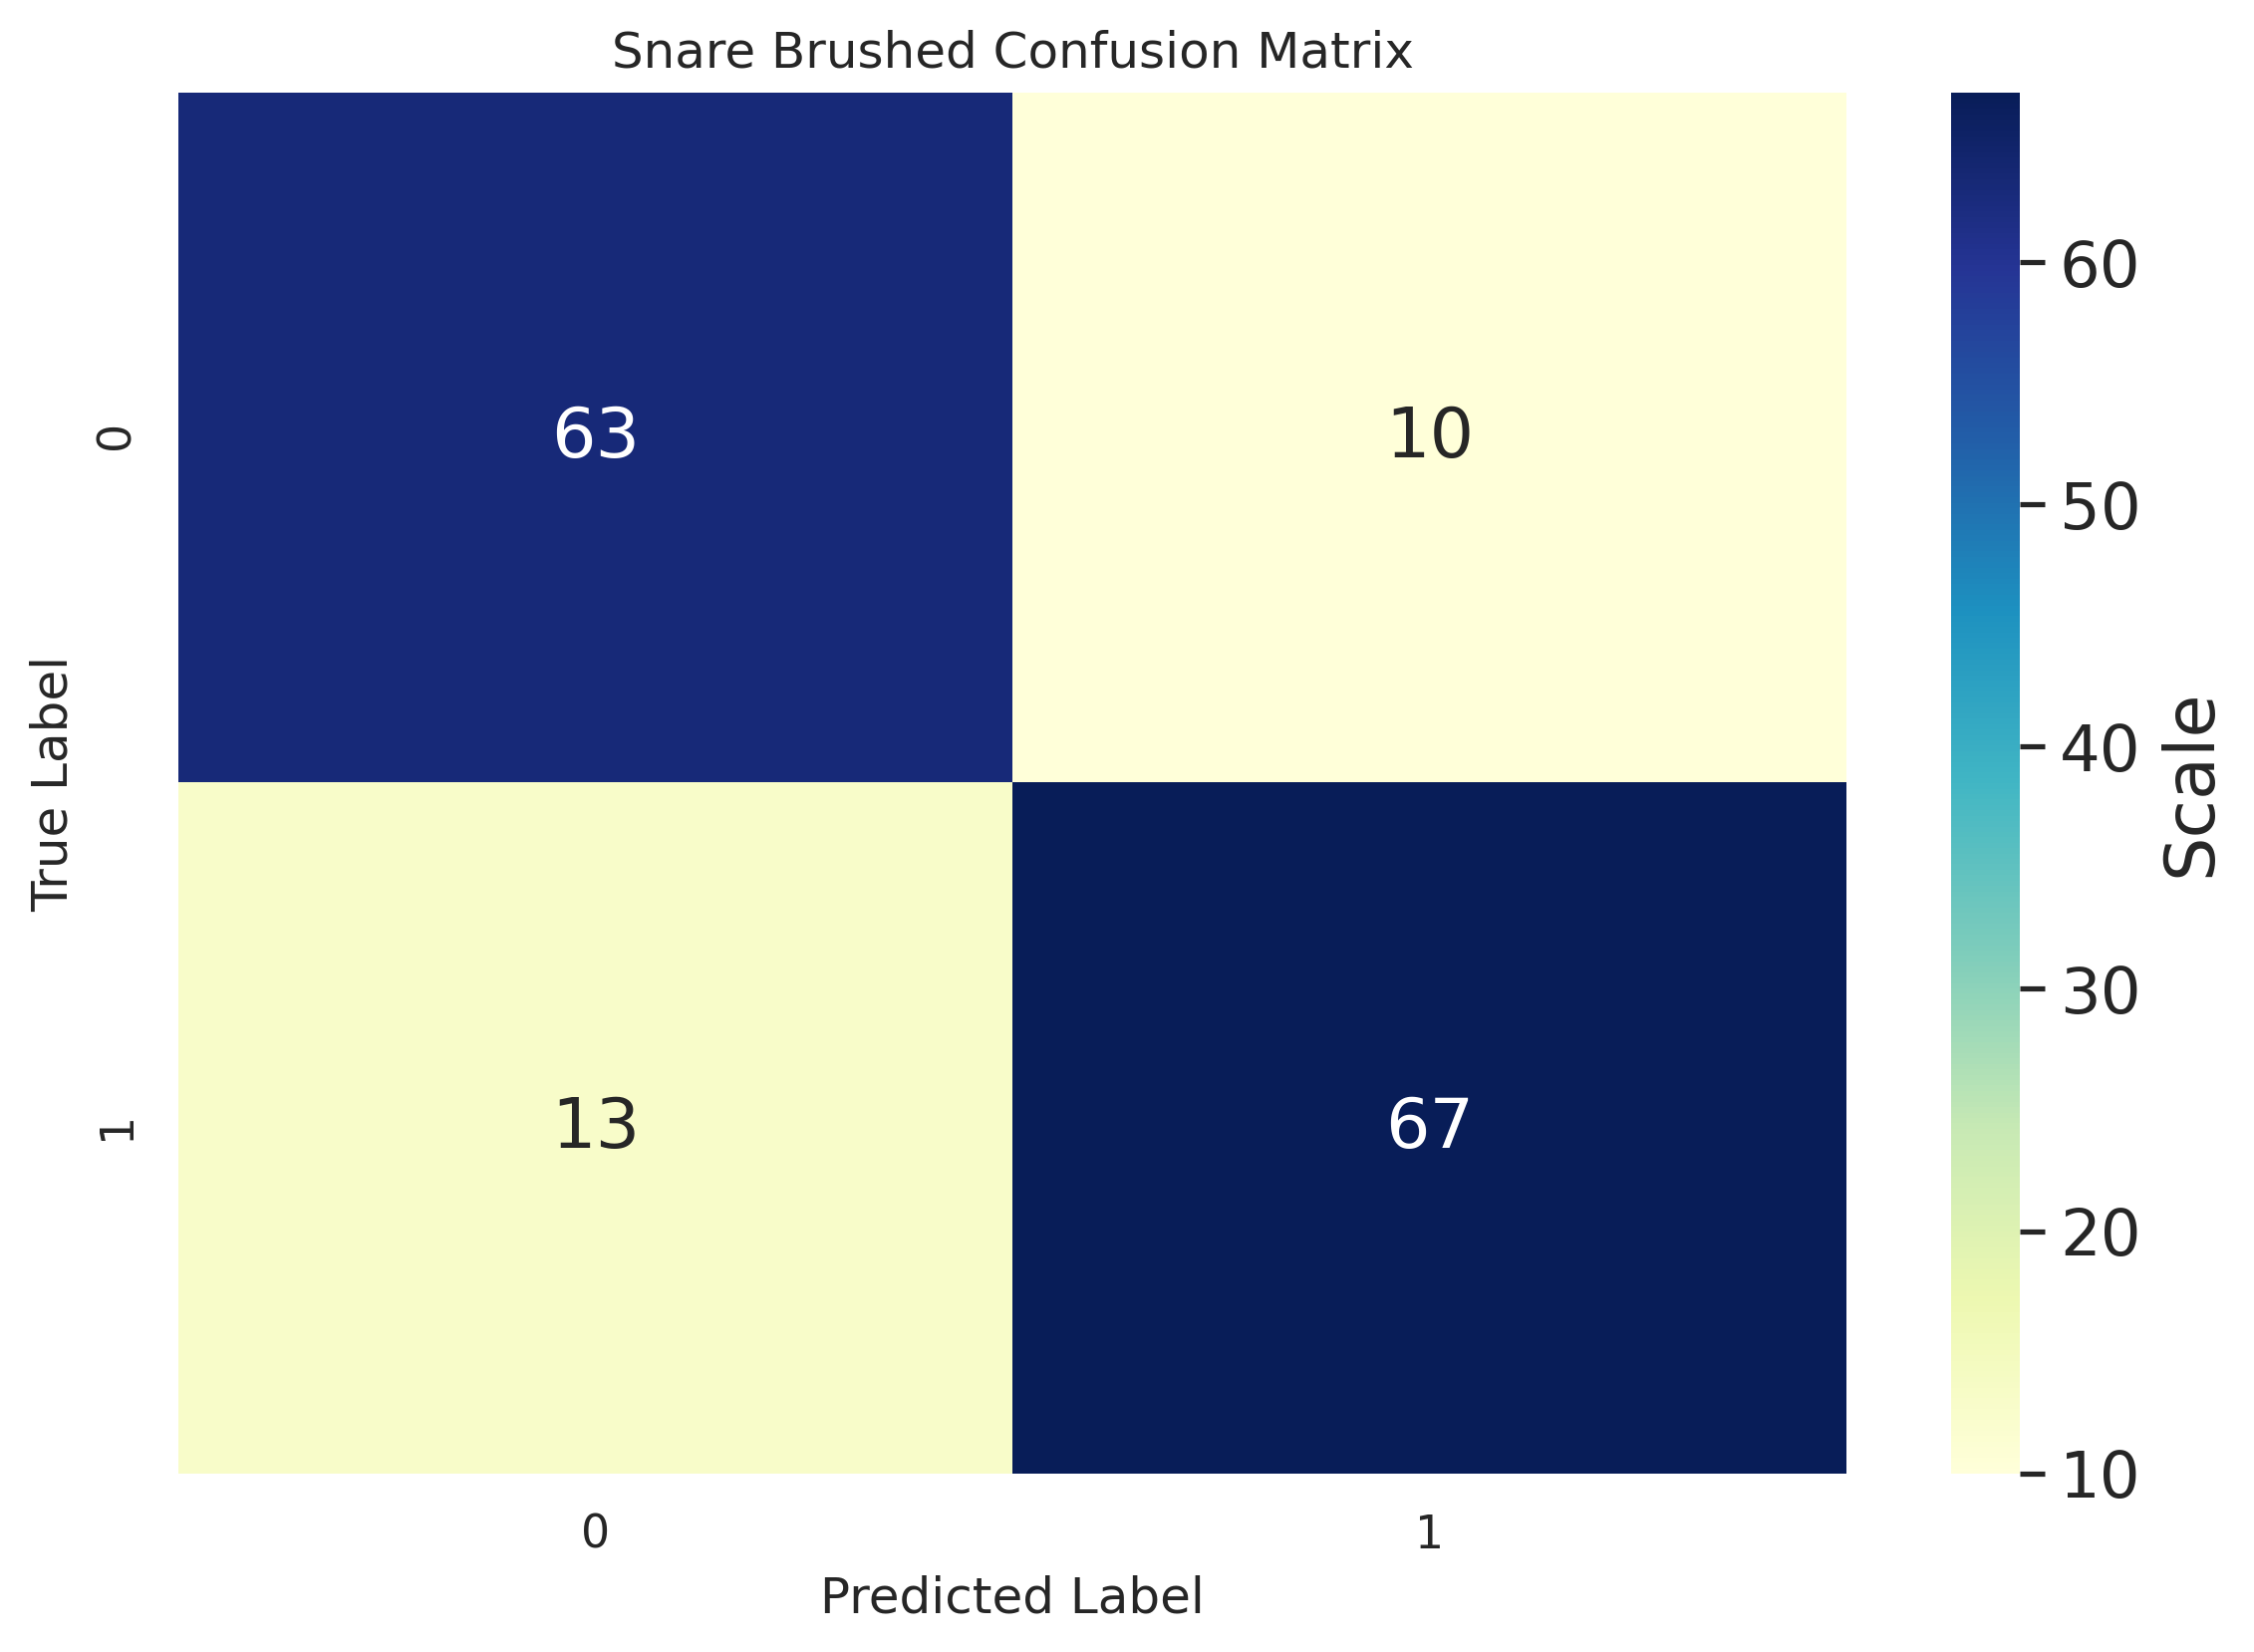
\includegraphics[width=\linewidth]{./immagini/first_classification/sn_brushed_cm.png}
		\caption{Matrice di confusione per il rullante spazzolato}
		\label{fig:cm_1b}
	\end{subfigure}
	
	\begin{subfigure}{.5\linewidth}
		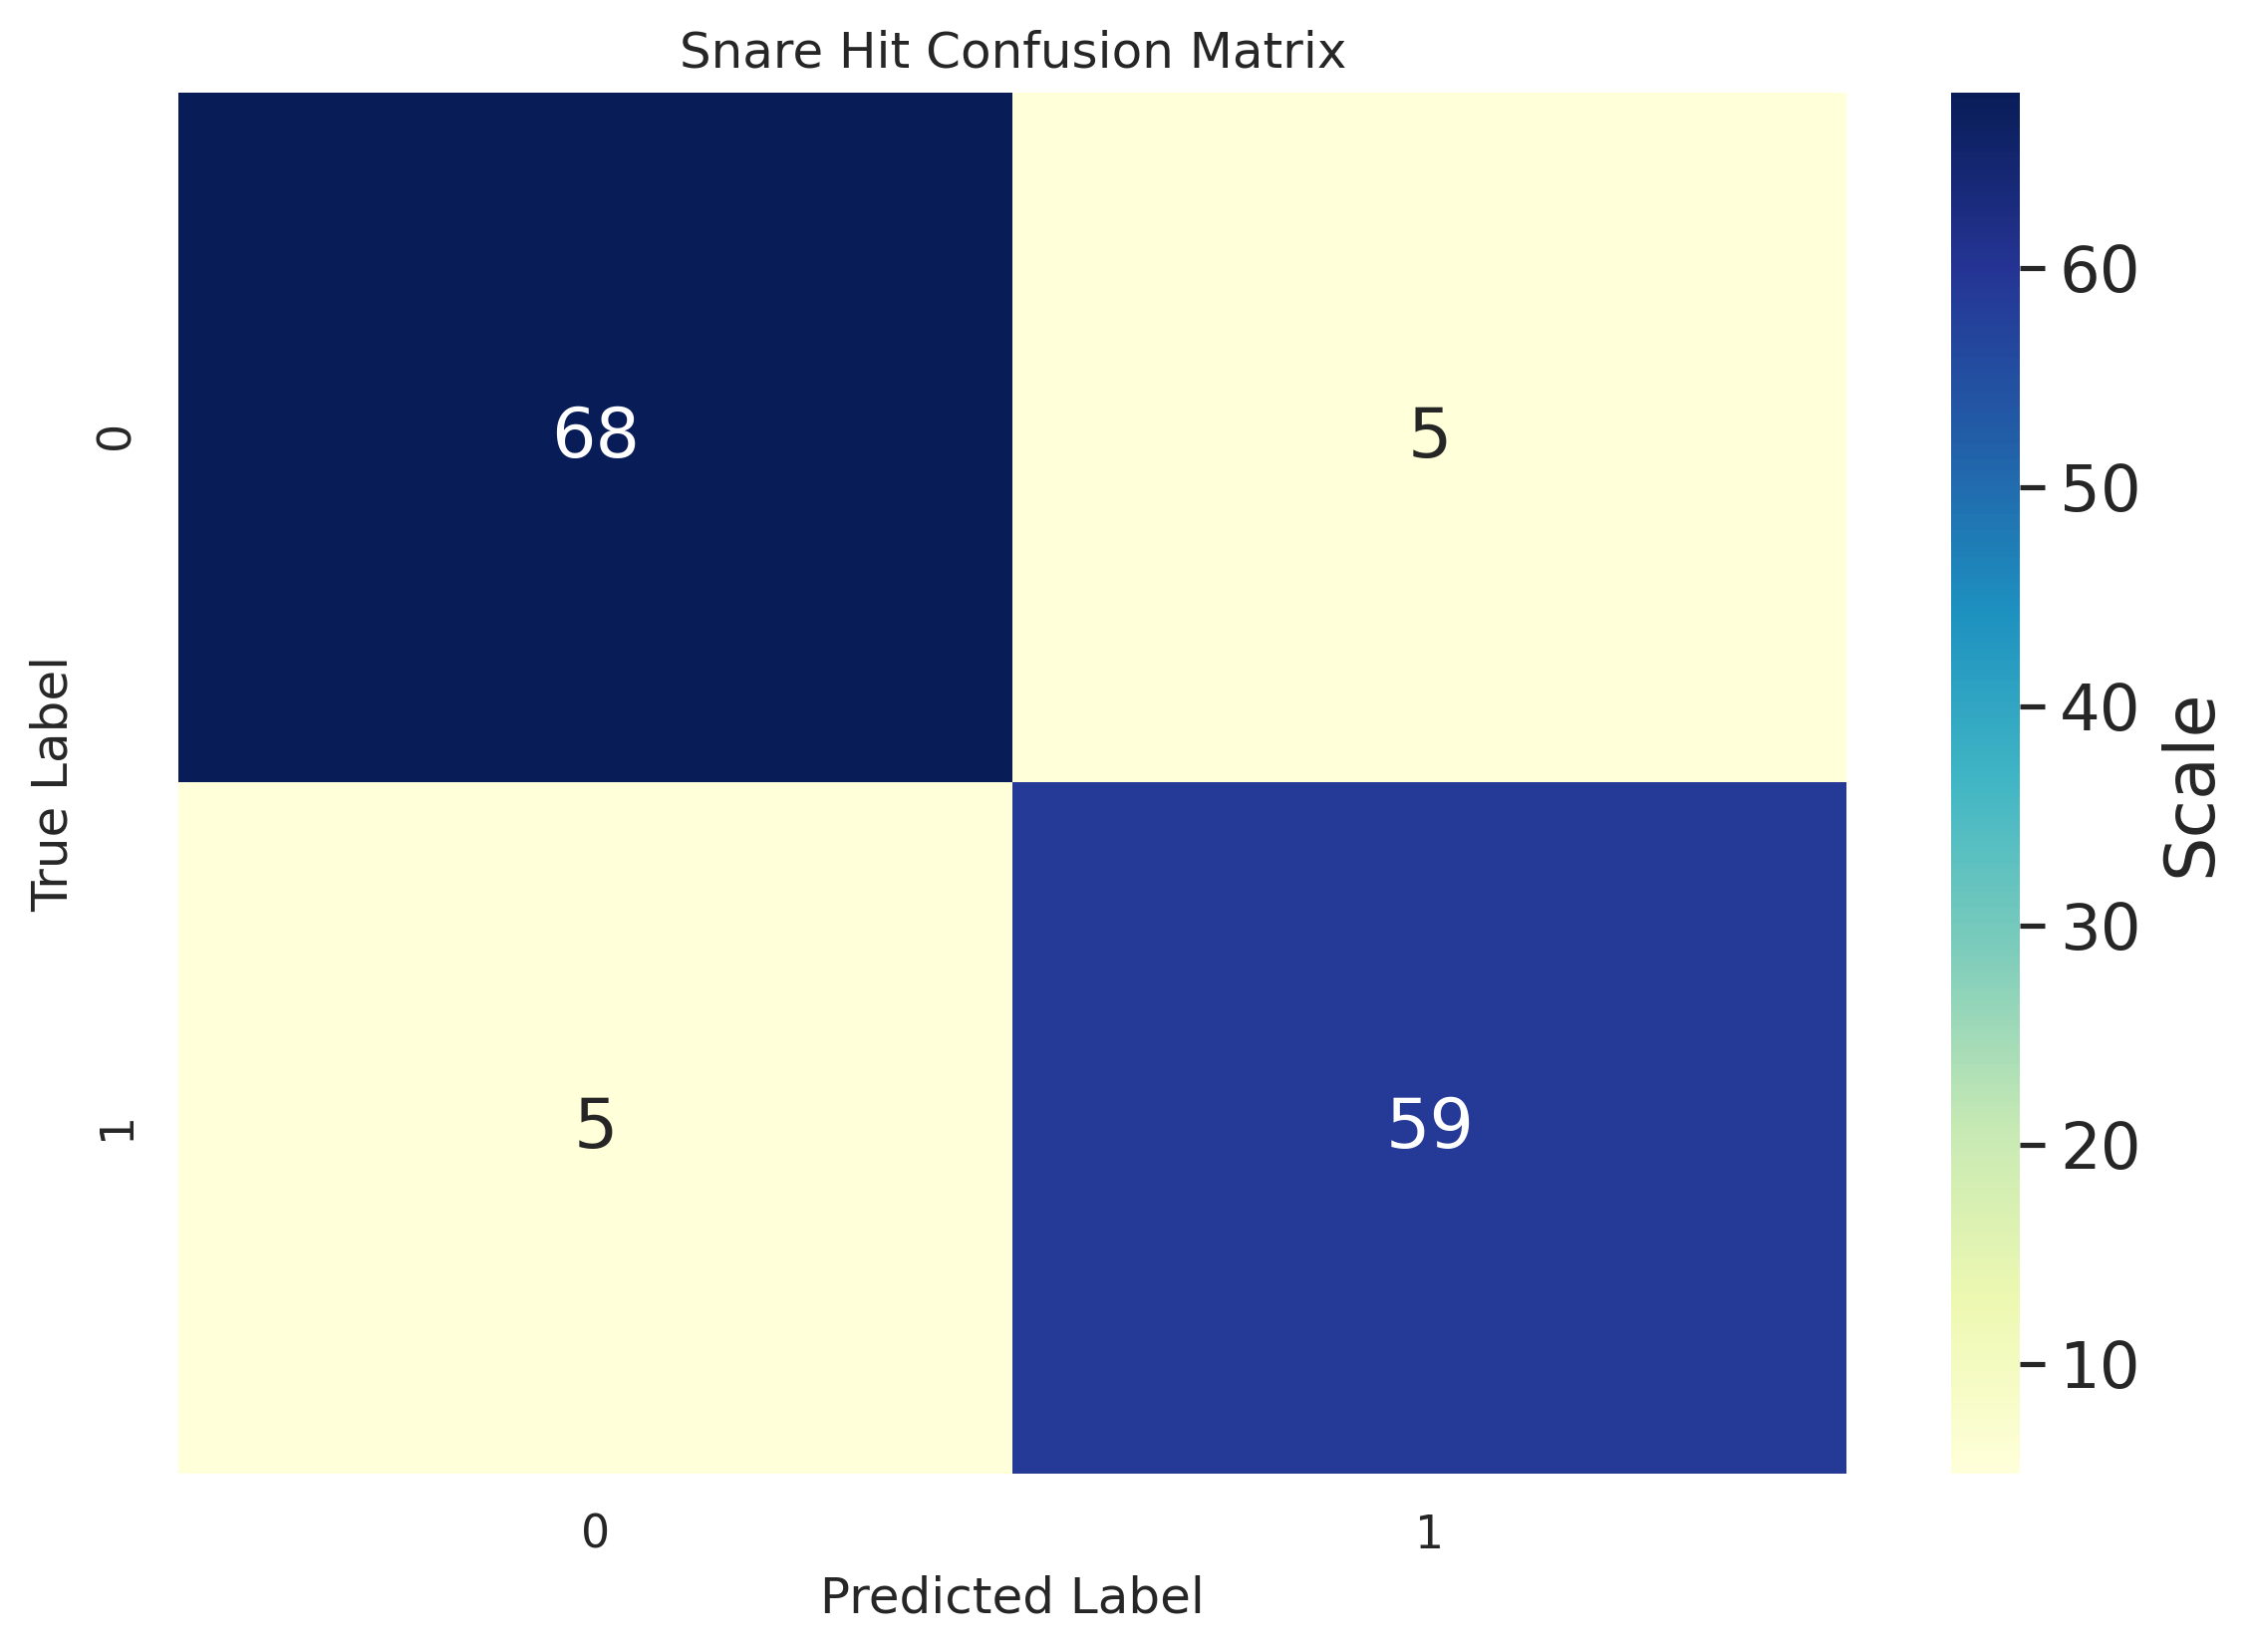
\includegraphics[width=\linewidth]{./immagini/first_classification/sn_hit_cm.png}
		\caption{Matrice di confusione per il colpo di rullante}
		\label{fig:cm_1c}
	\end{subfigure}\hfill
	\begin{subfigure}{.5\linewidth}
		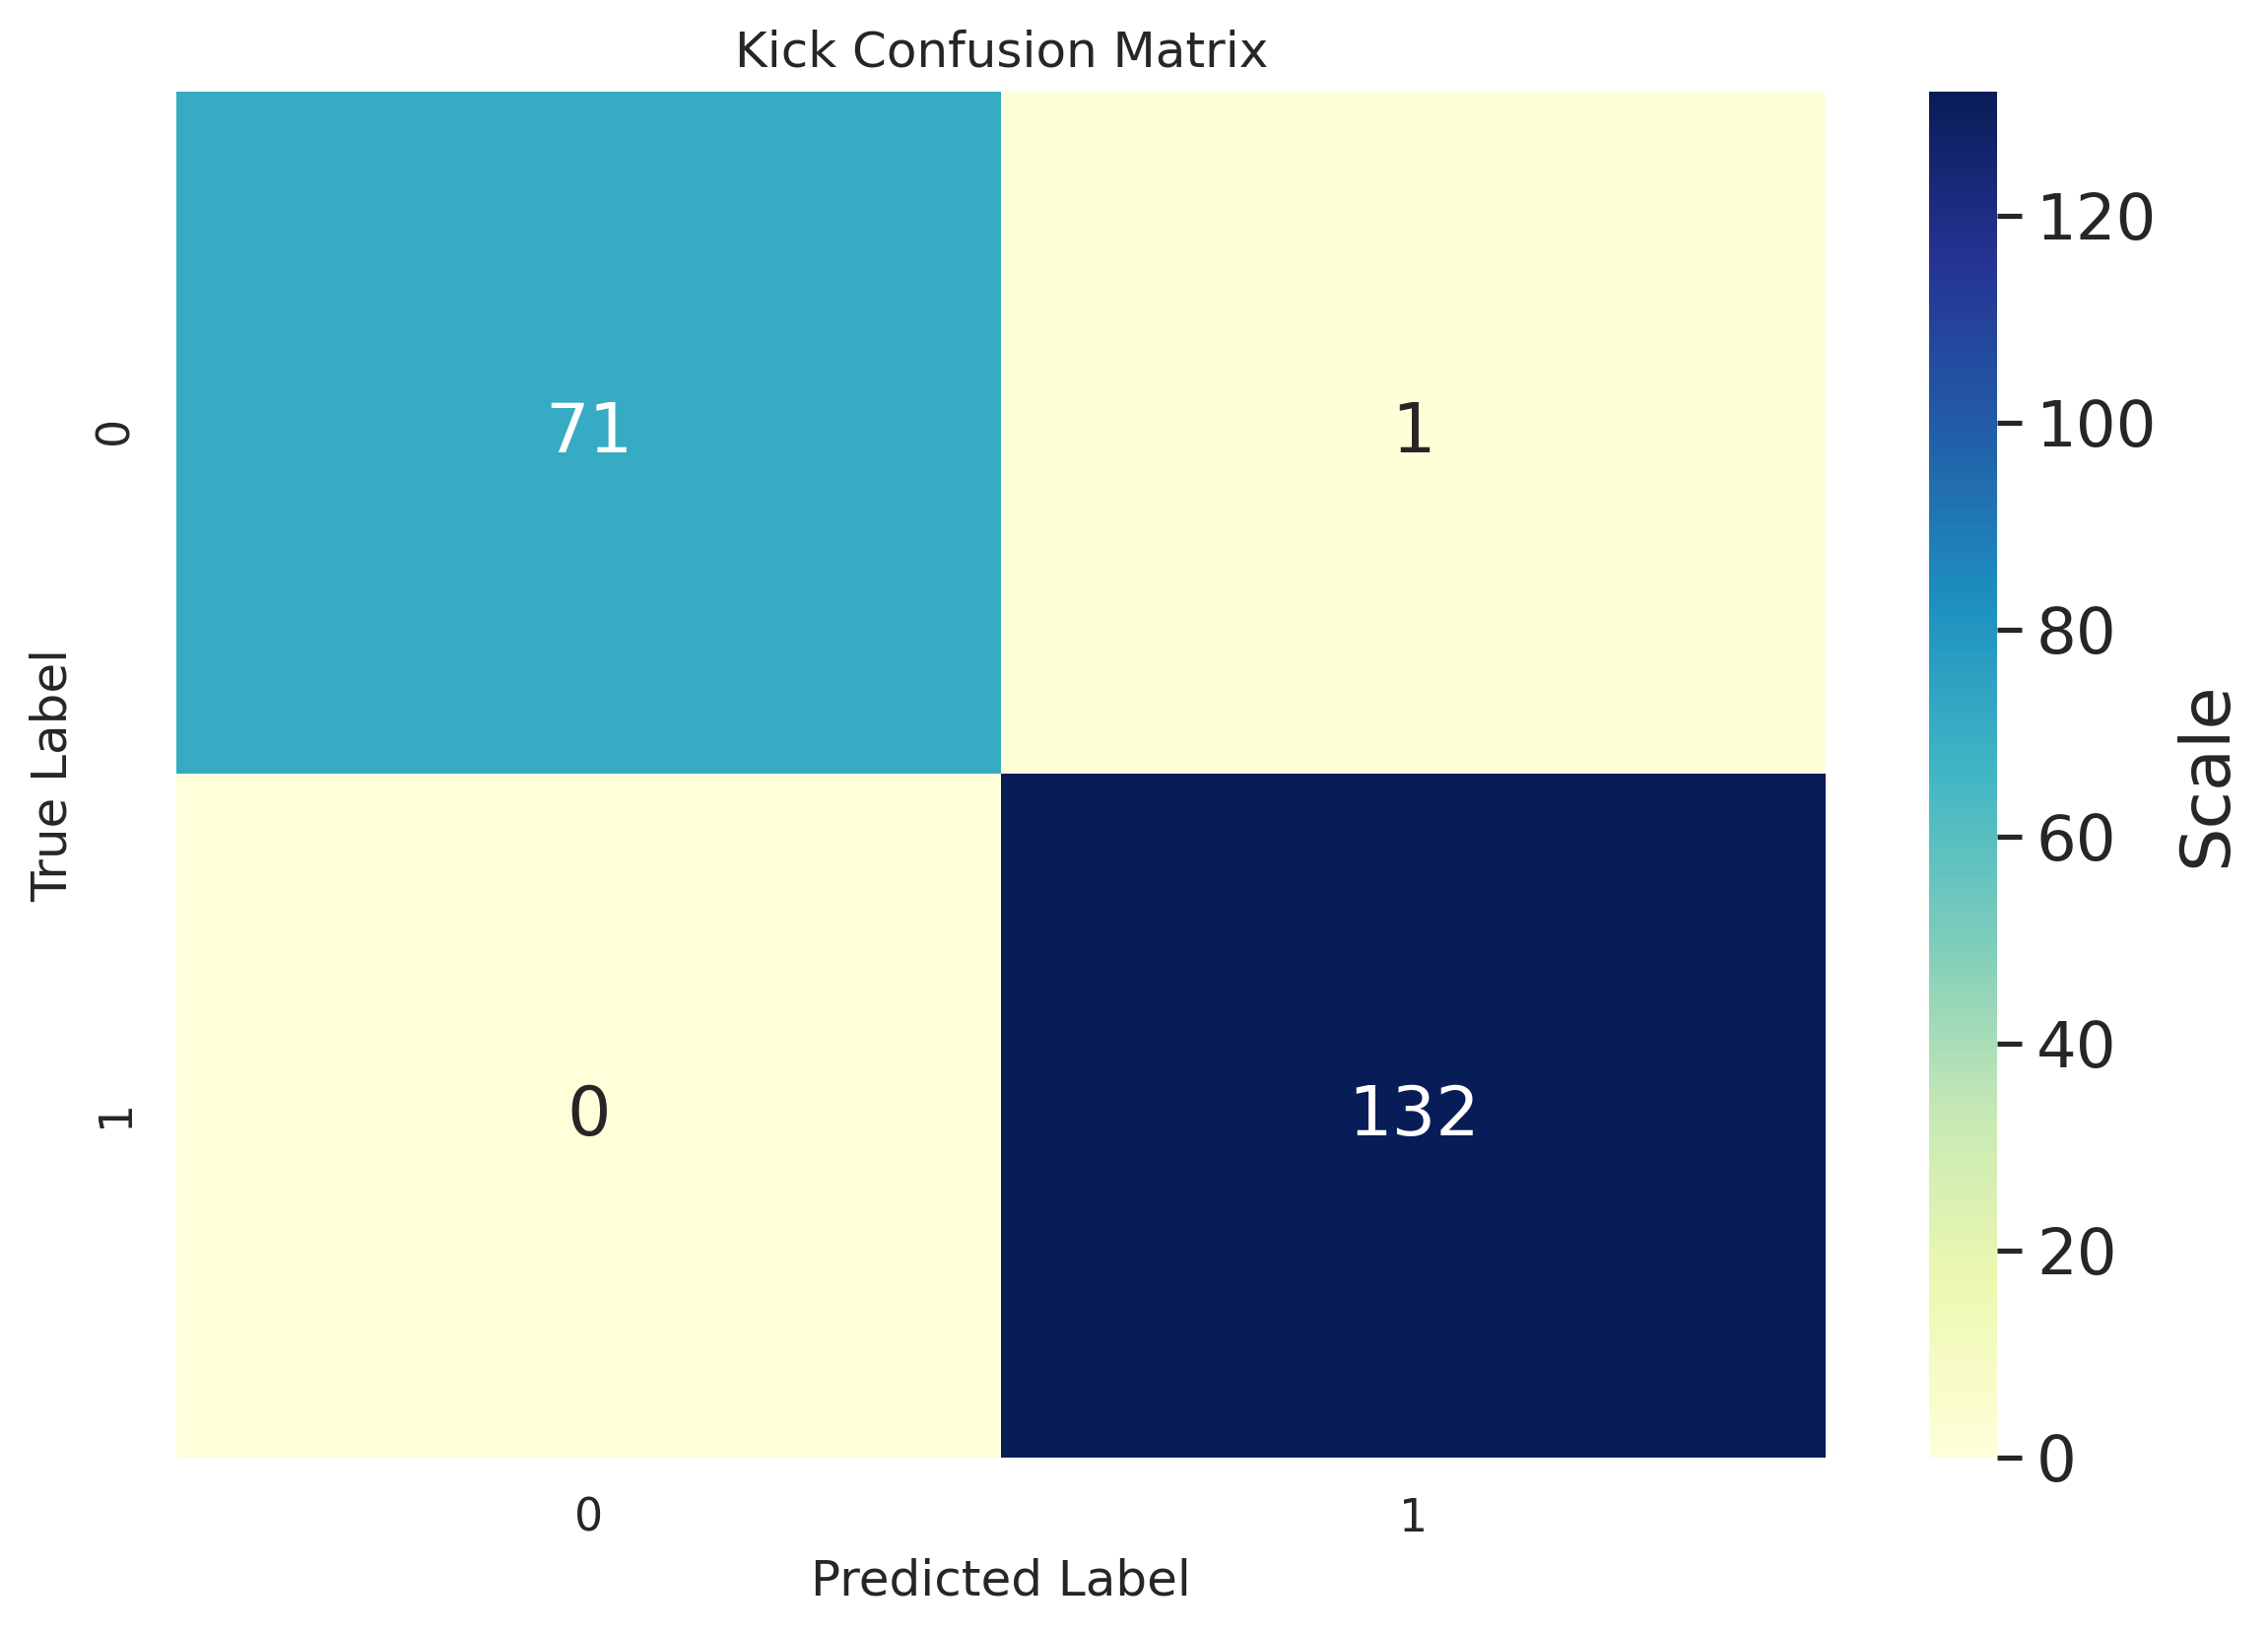
\includegraphics[width=\linewidth]{./immagini/first_classification/kick_cm.png}
		\caption{Matrice di confusione per la cassa}
		\label{fig:cm_1d}
	\end{subfigure}
	\caption{Matrici di confusione della prima fase}
	\label{fig:cm_1}
\end{figure}

Osservando dunque numerosità dei dati e risultati delle matrici di confusione possiamo dunque valutare la qualità dei risultati ottenuti calcolando l'accuracy \ref{formula:accuracy}, TPR\ref{formula:sensitivity} e TNR\ref{formula:specificity}

\begin{table}[h!]
	\begin{center}
		\begin{tabular}{l|c|c|r} % <-- Alignments: 1st column left, 2nd middle and 3rd right, with vertical lines in between
			\textbf{Classe} & \textbf{ACC} & \textbf{TPR} & \textbf{TNR} \\
			%$\alpha$ & $\beta$ & $\gamma$ \\
			\hline
			Basso & 0.92 & 0.94 & 0.90\\
			Spazzolata di Rullante & 0.85 & 0.84 & 0.86\\
			Colpo di Rullante & 0.93 & 0.92 & 0.93\\
			Cassa & 0.99 & 1.00 & 0.99
		\end{tabular}
		\caption{Metriche di valutazione prima fase.}
		\label{tab:accuracy_1}
	\end{center}
\end{table}

È possibile notare degli ottimi risultati per tutti gli strumenti nel riconoscimento, in particolar modo per la cassa e il colpo di rullante, vista la natura dell'onda sonora da loro prodotta, un'impulso con una crescita molto rapida. Lo strumento che è riconosciuto peggio è invece il rullante spazzolato, anch'esso per la natura dell'onda sonora da lui prodotto, meno distinguibile da un possibile rumore per ampiezza d'onda e impulso con crescita molto minore.\\
Essendo questi risultati molto buoni, è possibile affermare che con le features utilizzate risulta possibile distinguere tra una nota e una non nota, e dunque passare a una fase di riconoscimento più fine illustrata nella sezione che segue.\\

\section{Seconda fase}
In questa fase si vuole rendere più fine il riconoscimento delle note, consentendo di accettare in input un'intera traccia audio e non solo dei singoli frammenti di note o non per il riconoscimento. Partendo dalla classificazione, viene sempre utilizzato J48 per costruire un albero di decisione che non porterà più a decidere se un frammento analizzato è una nota o meno, questo infatti porterà a classificare in 5 classi diverse ogni elemento di input, come appunto descritto a inizio capitolo. L'algoritmo di classificazione è molto simile al passo precedente, l'unica differenza è che vengono scelti dei campioni più lunghi per poter essere spezzati in più sub-campioni, il primo classificato come 5 (certamente una nota), l'ultimo come 1 (certamente non una nota). Ogni sub-campione avrà la stessa lunghezza, e proprio così facendo è stato possibile fornire in input delle intere tracce, perché suddivise in sub-campioni, di lunghezza costante, al quale si associa a ognuno una classe da 1 a 5 che consente così di localizzare temporalmente le note, e risolvere dunque il problema posto inizialmente.\\
%INSERISCI MATRICI DI CONFUSIONE

\begin{figure}[h!]
	\centering
	\begin{subfigure}{.5\linewidth}
		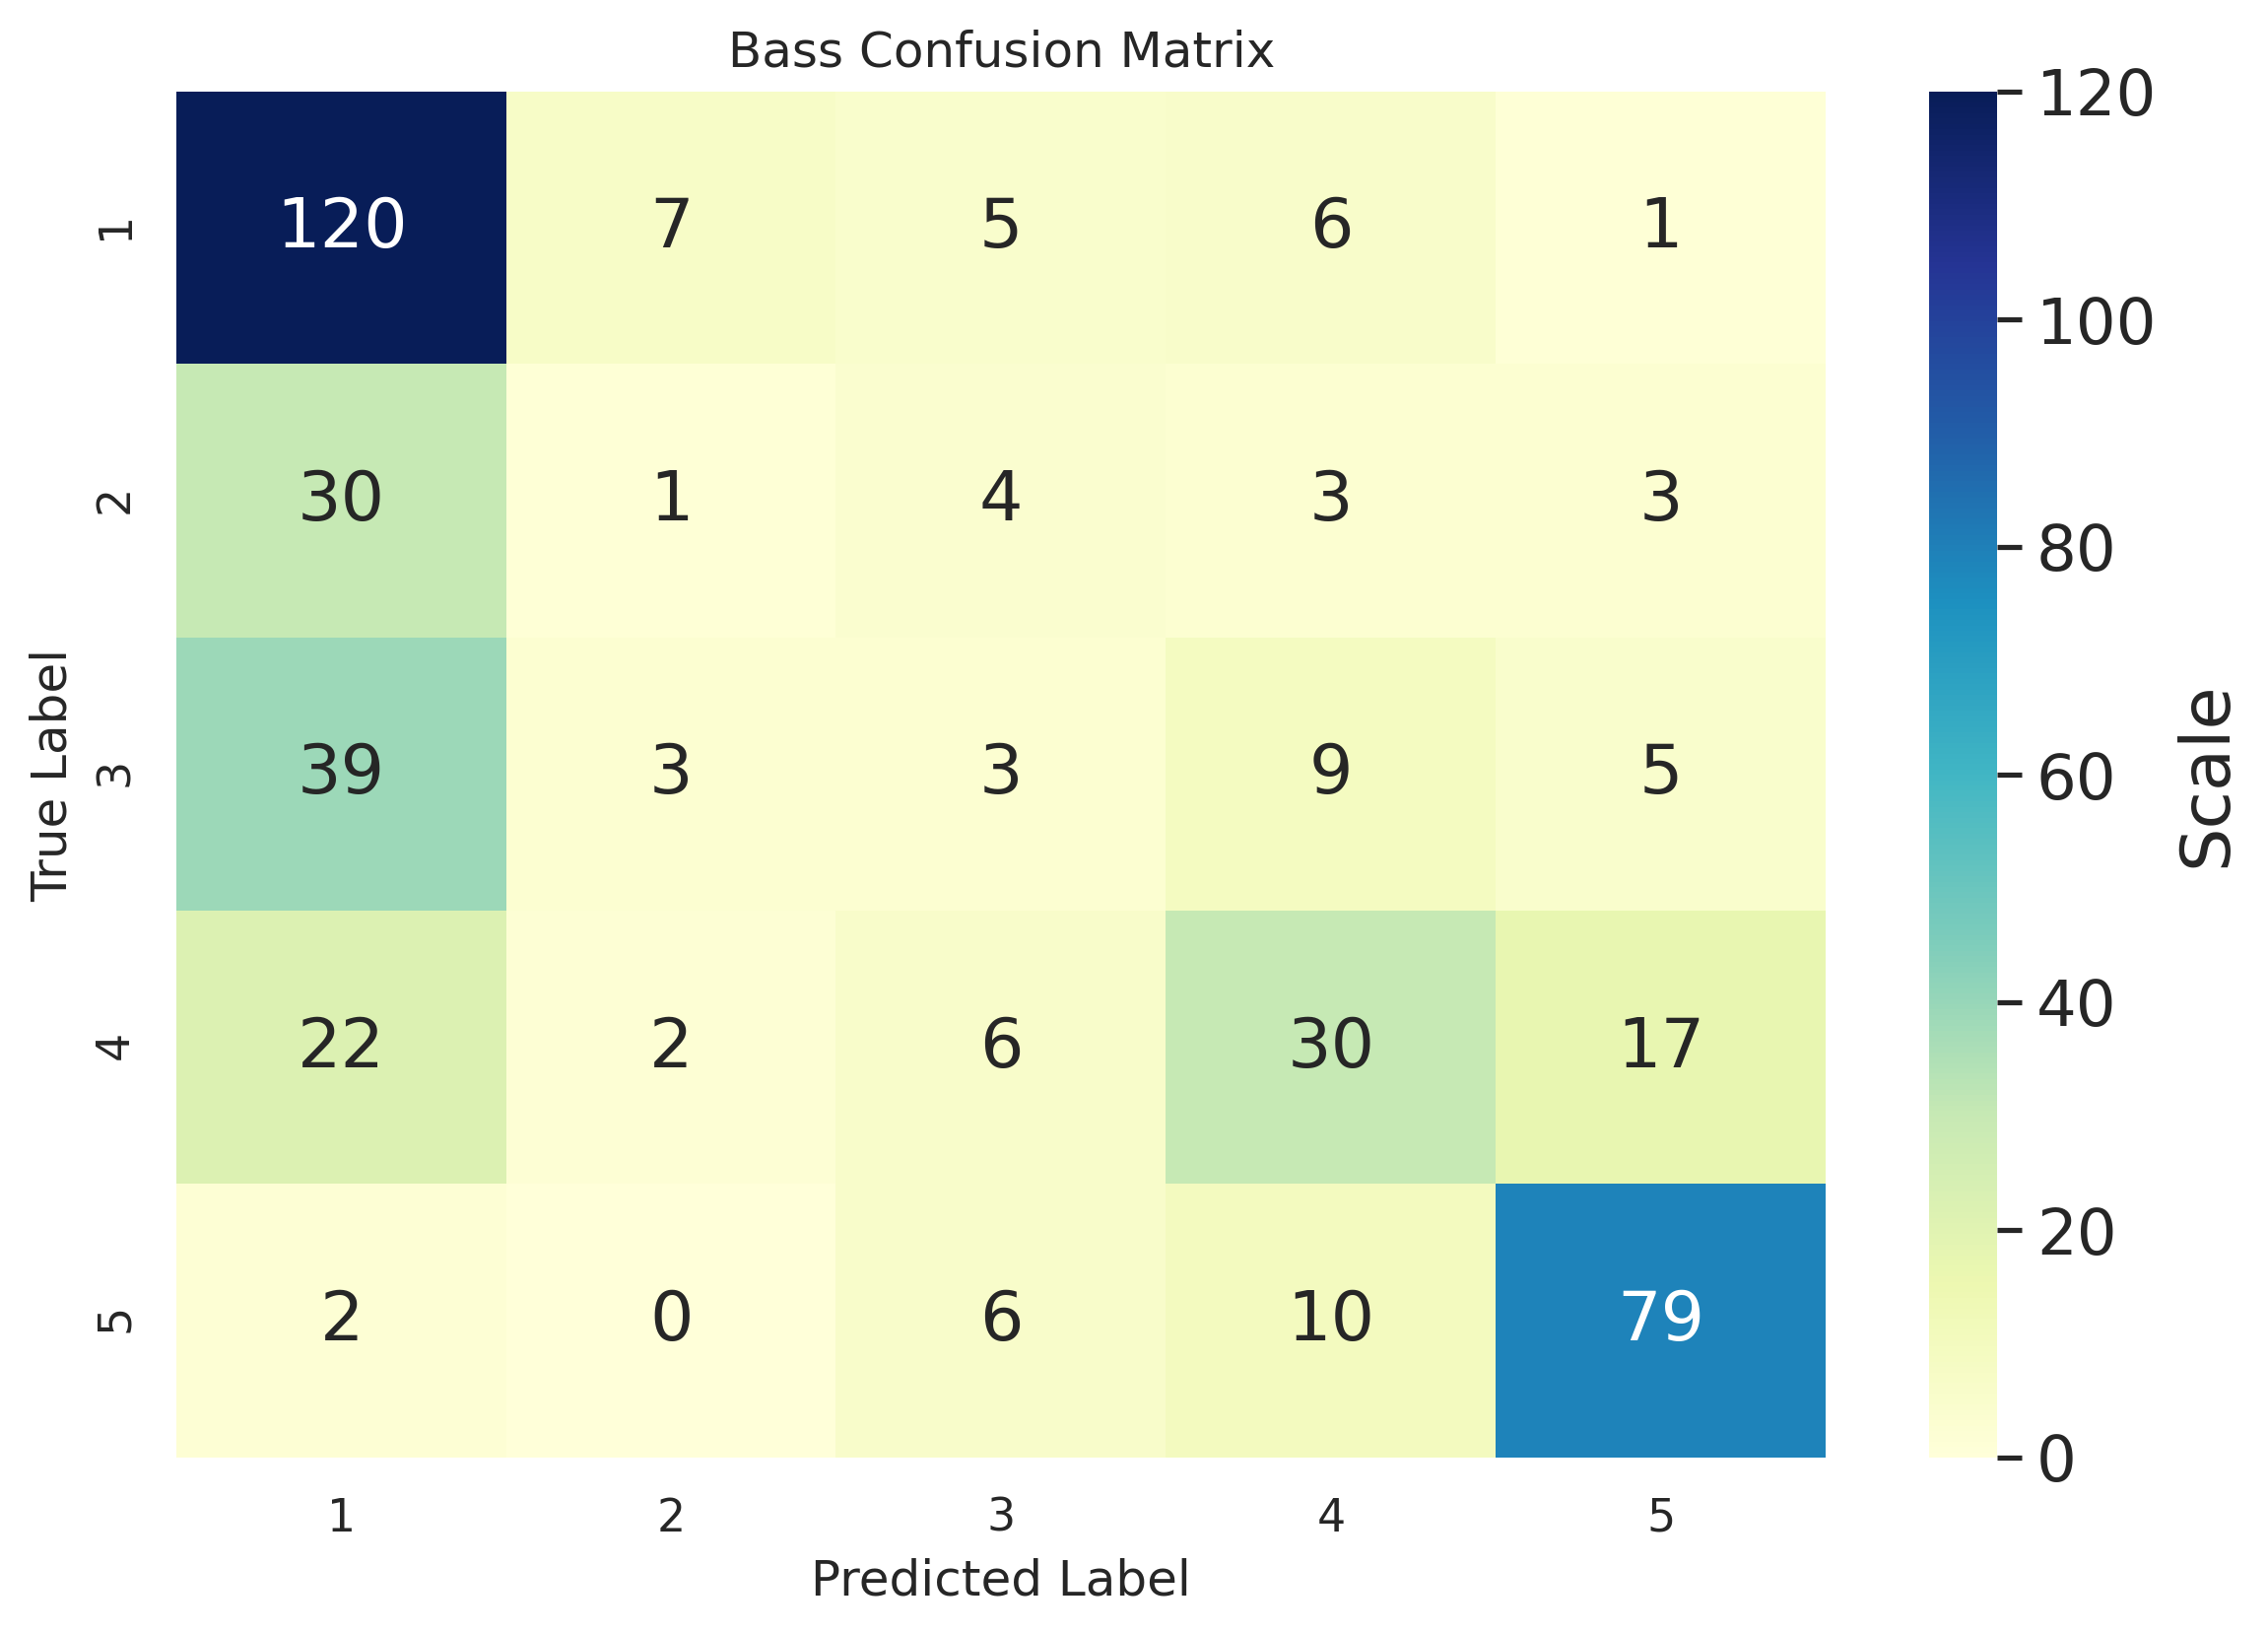
\includegraphics[width=\linewidth]{./immagini/second_classification/cb_cm.png} 
		\caption{Matrice di confusione per il basso}
		\label{fig:cm_2a}
	\end{subfigure}\hfill
	\begin{subfigure}{.5\linewidth}
		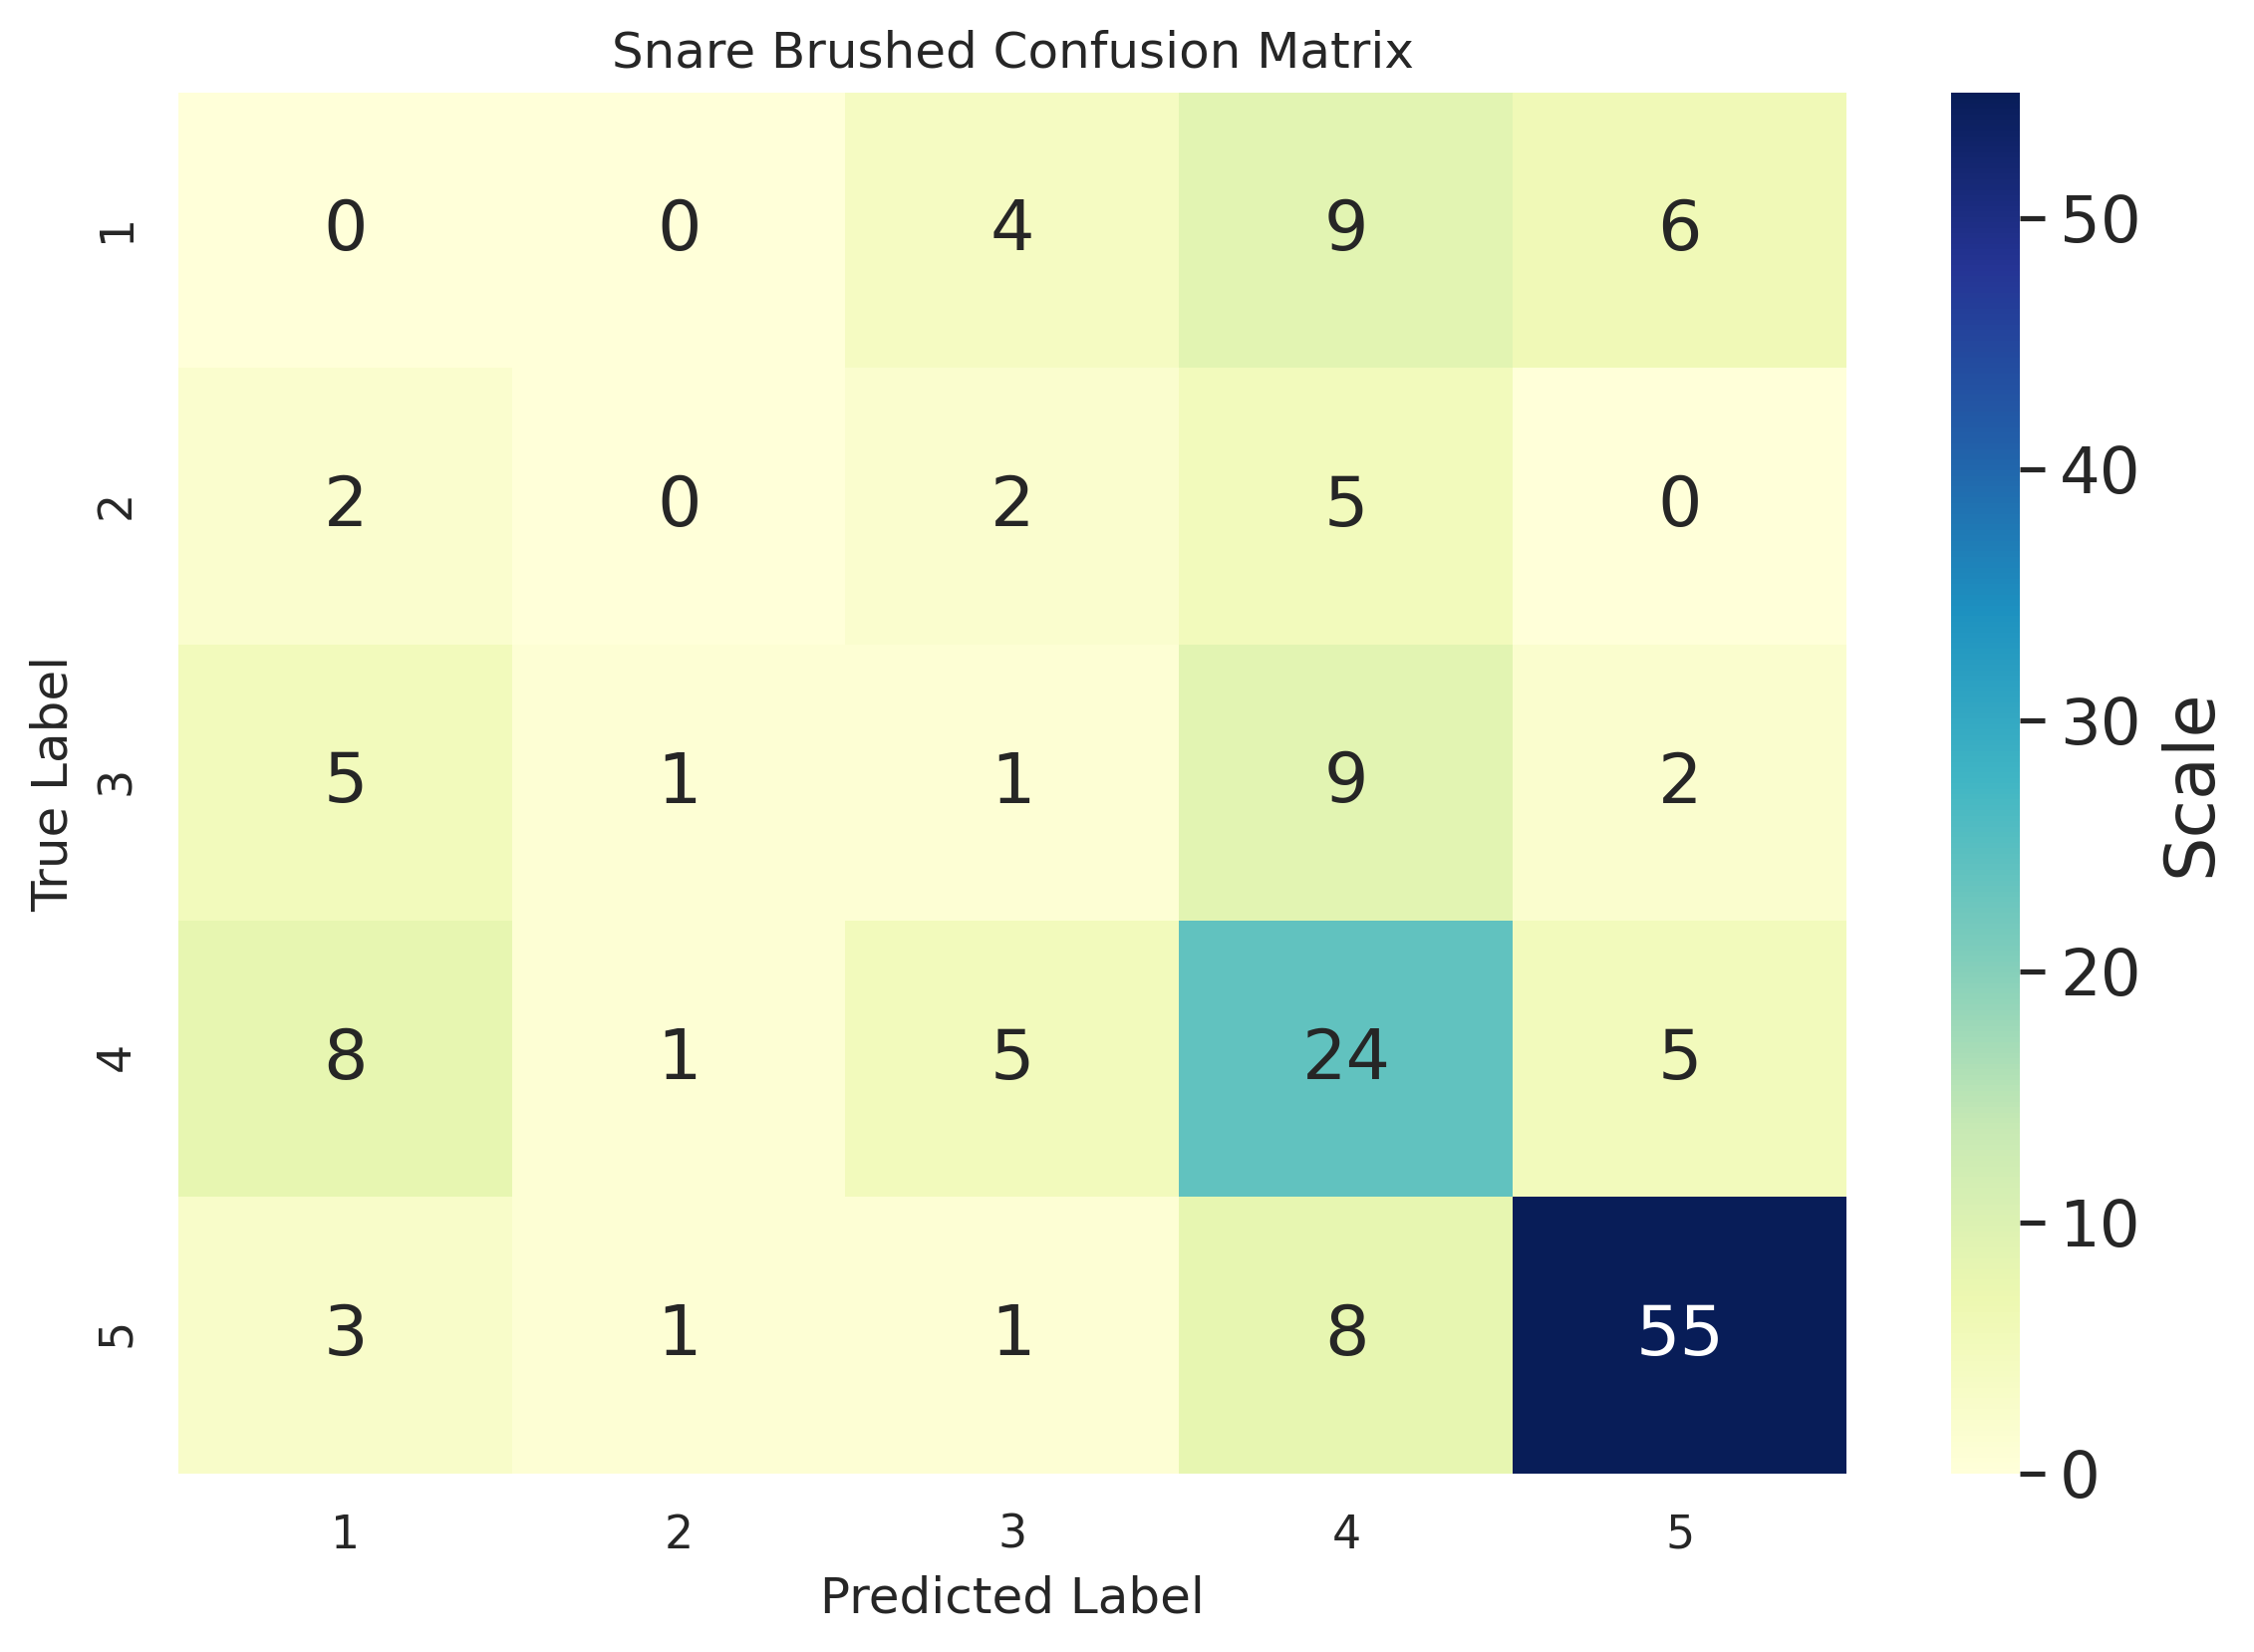
\includegraphics[width=\linewidth]{./immagini/second_classification/sn_brushed_cm.png}
		\caption{Matrice di confusione per il rullante spazzolato}
		\label{fig:cm_2b}
	\end{subfigure}
	
	\begin{subfigure}{.5\linewidth}
		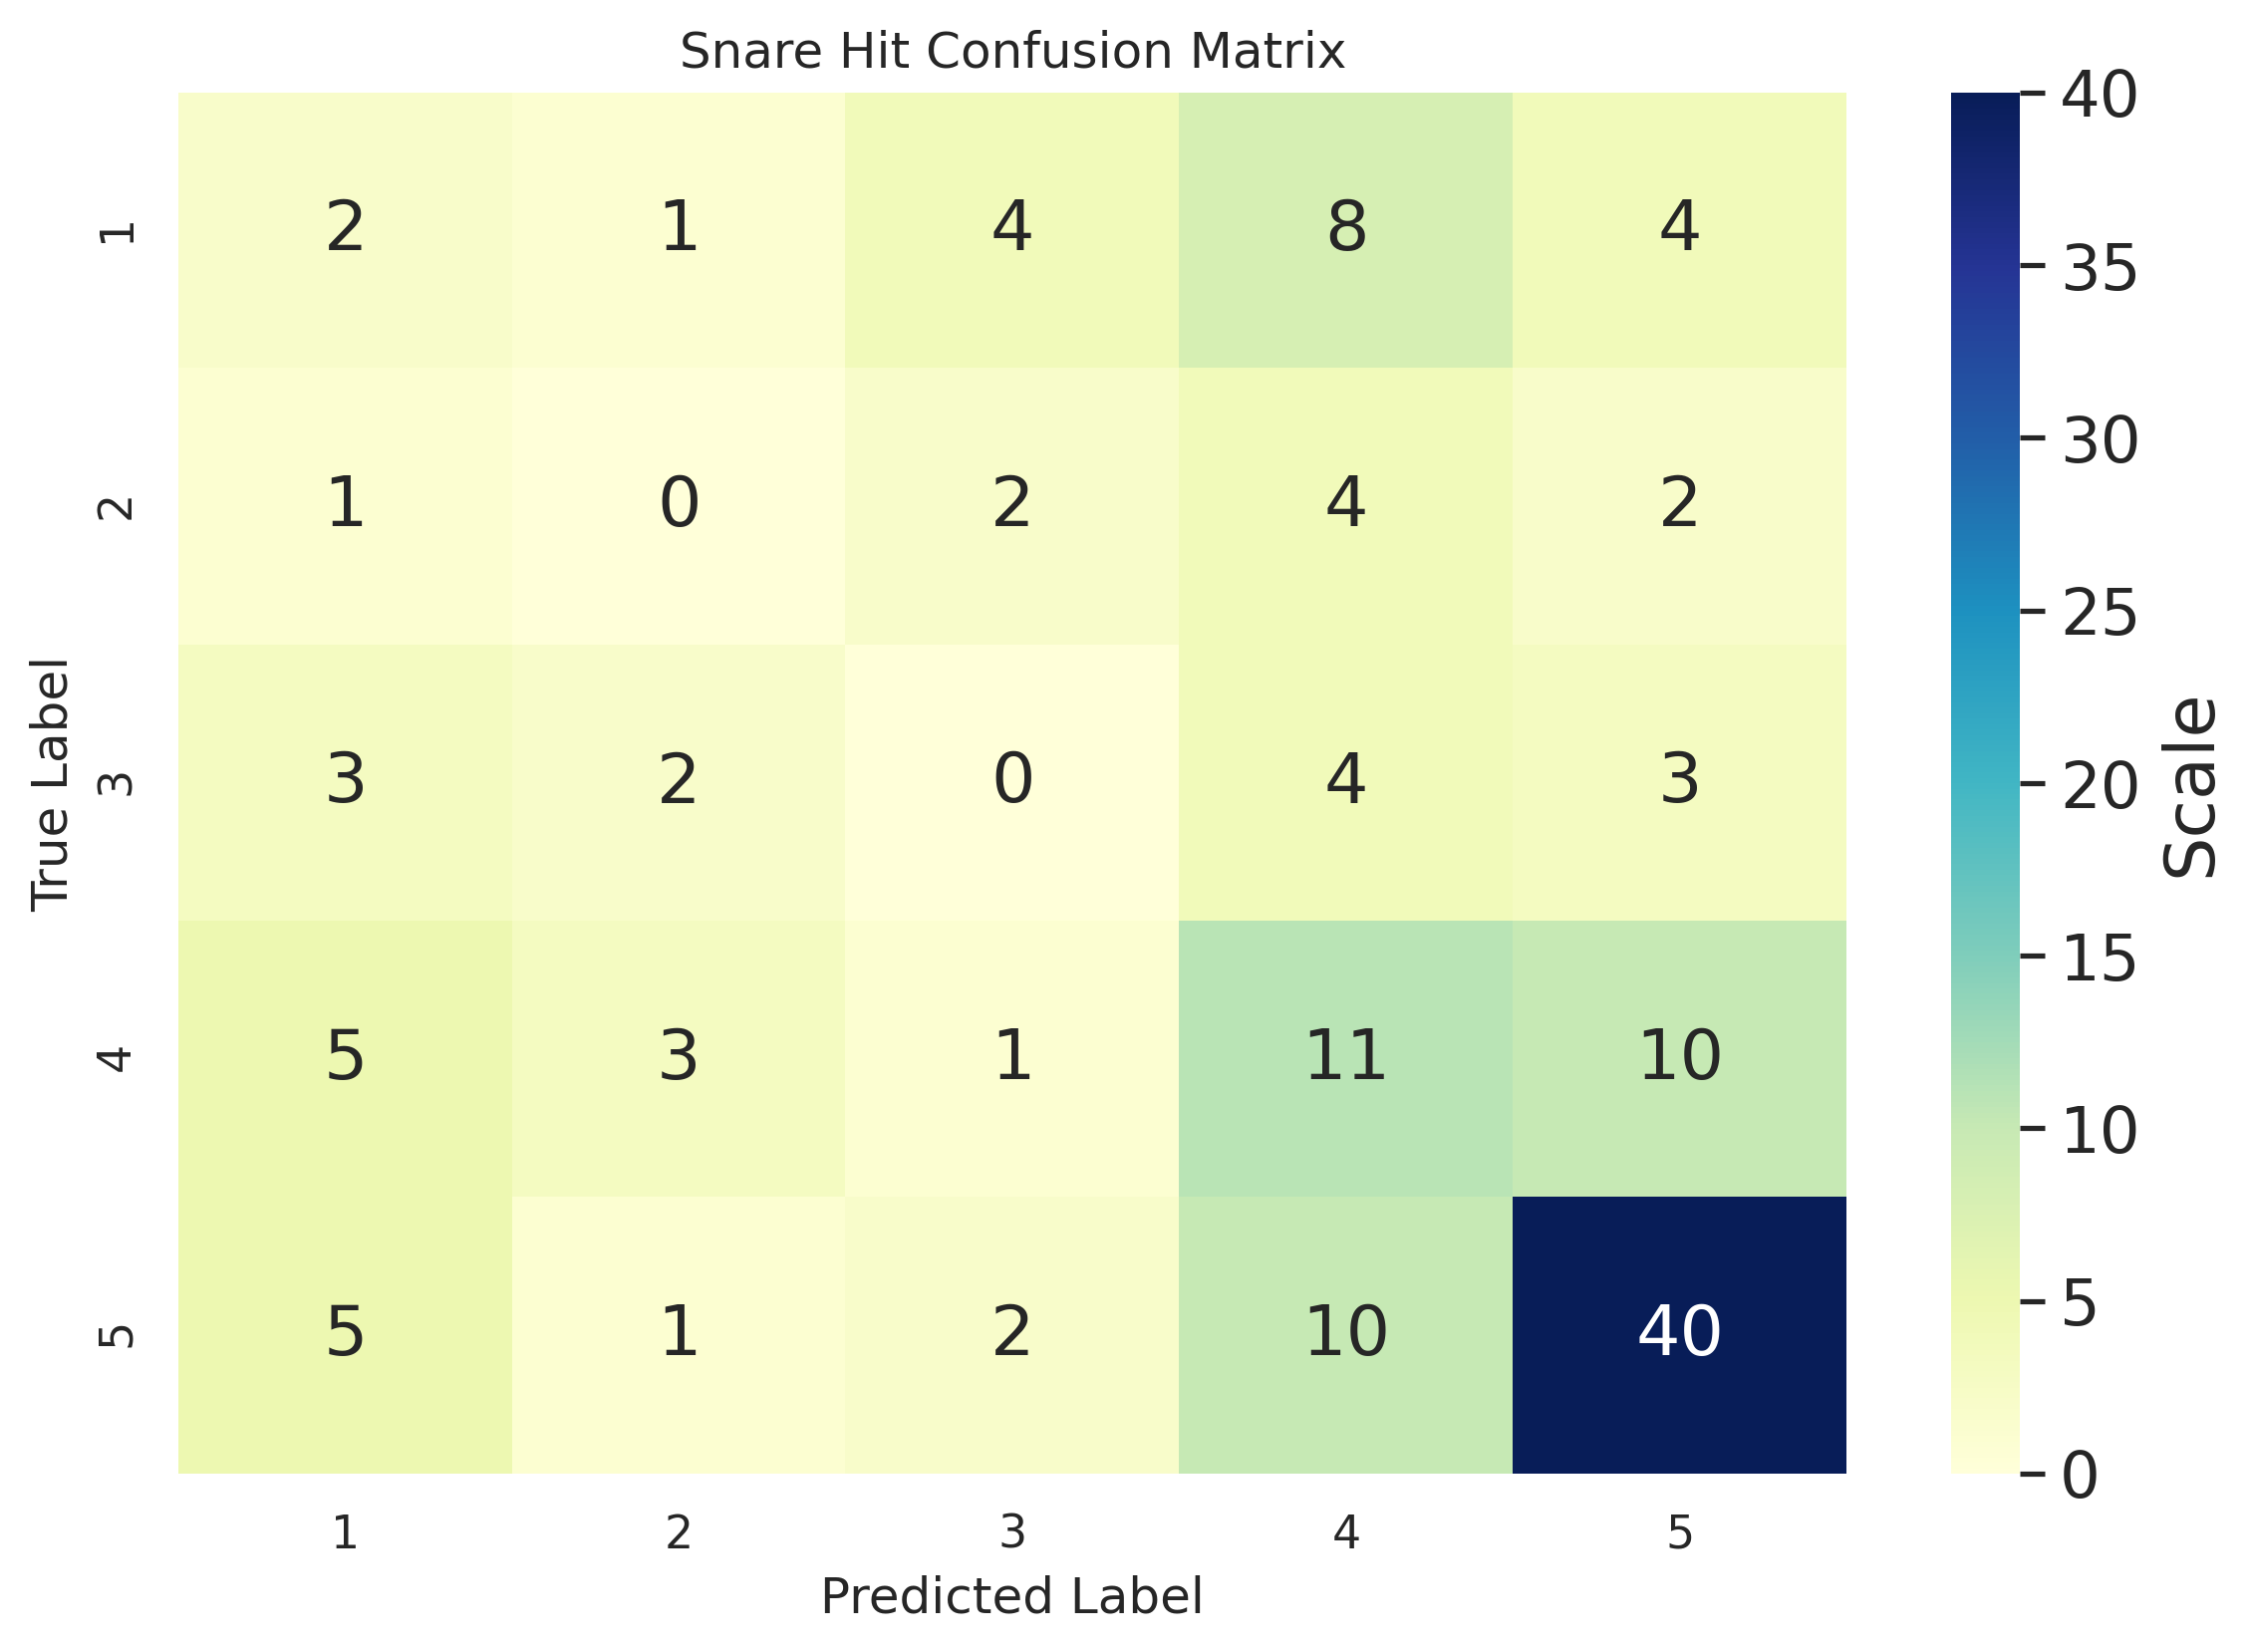
\includegraphics[width=\linewidth]{./immagini/second_classification/sn_hit_cm.png}
		\caption{Matrice di confusione per il colpo di rullante}
		\label{fig:cm_2c}
	\end{subfigure}\hfill
	\begin{subfigure}{.5\linewidth}
		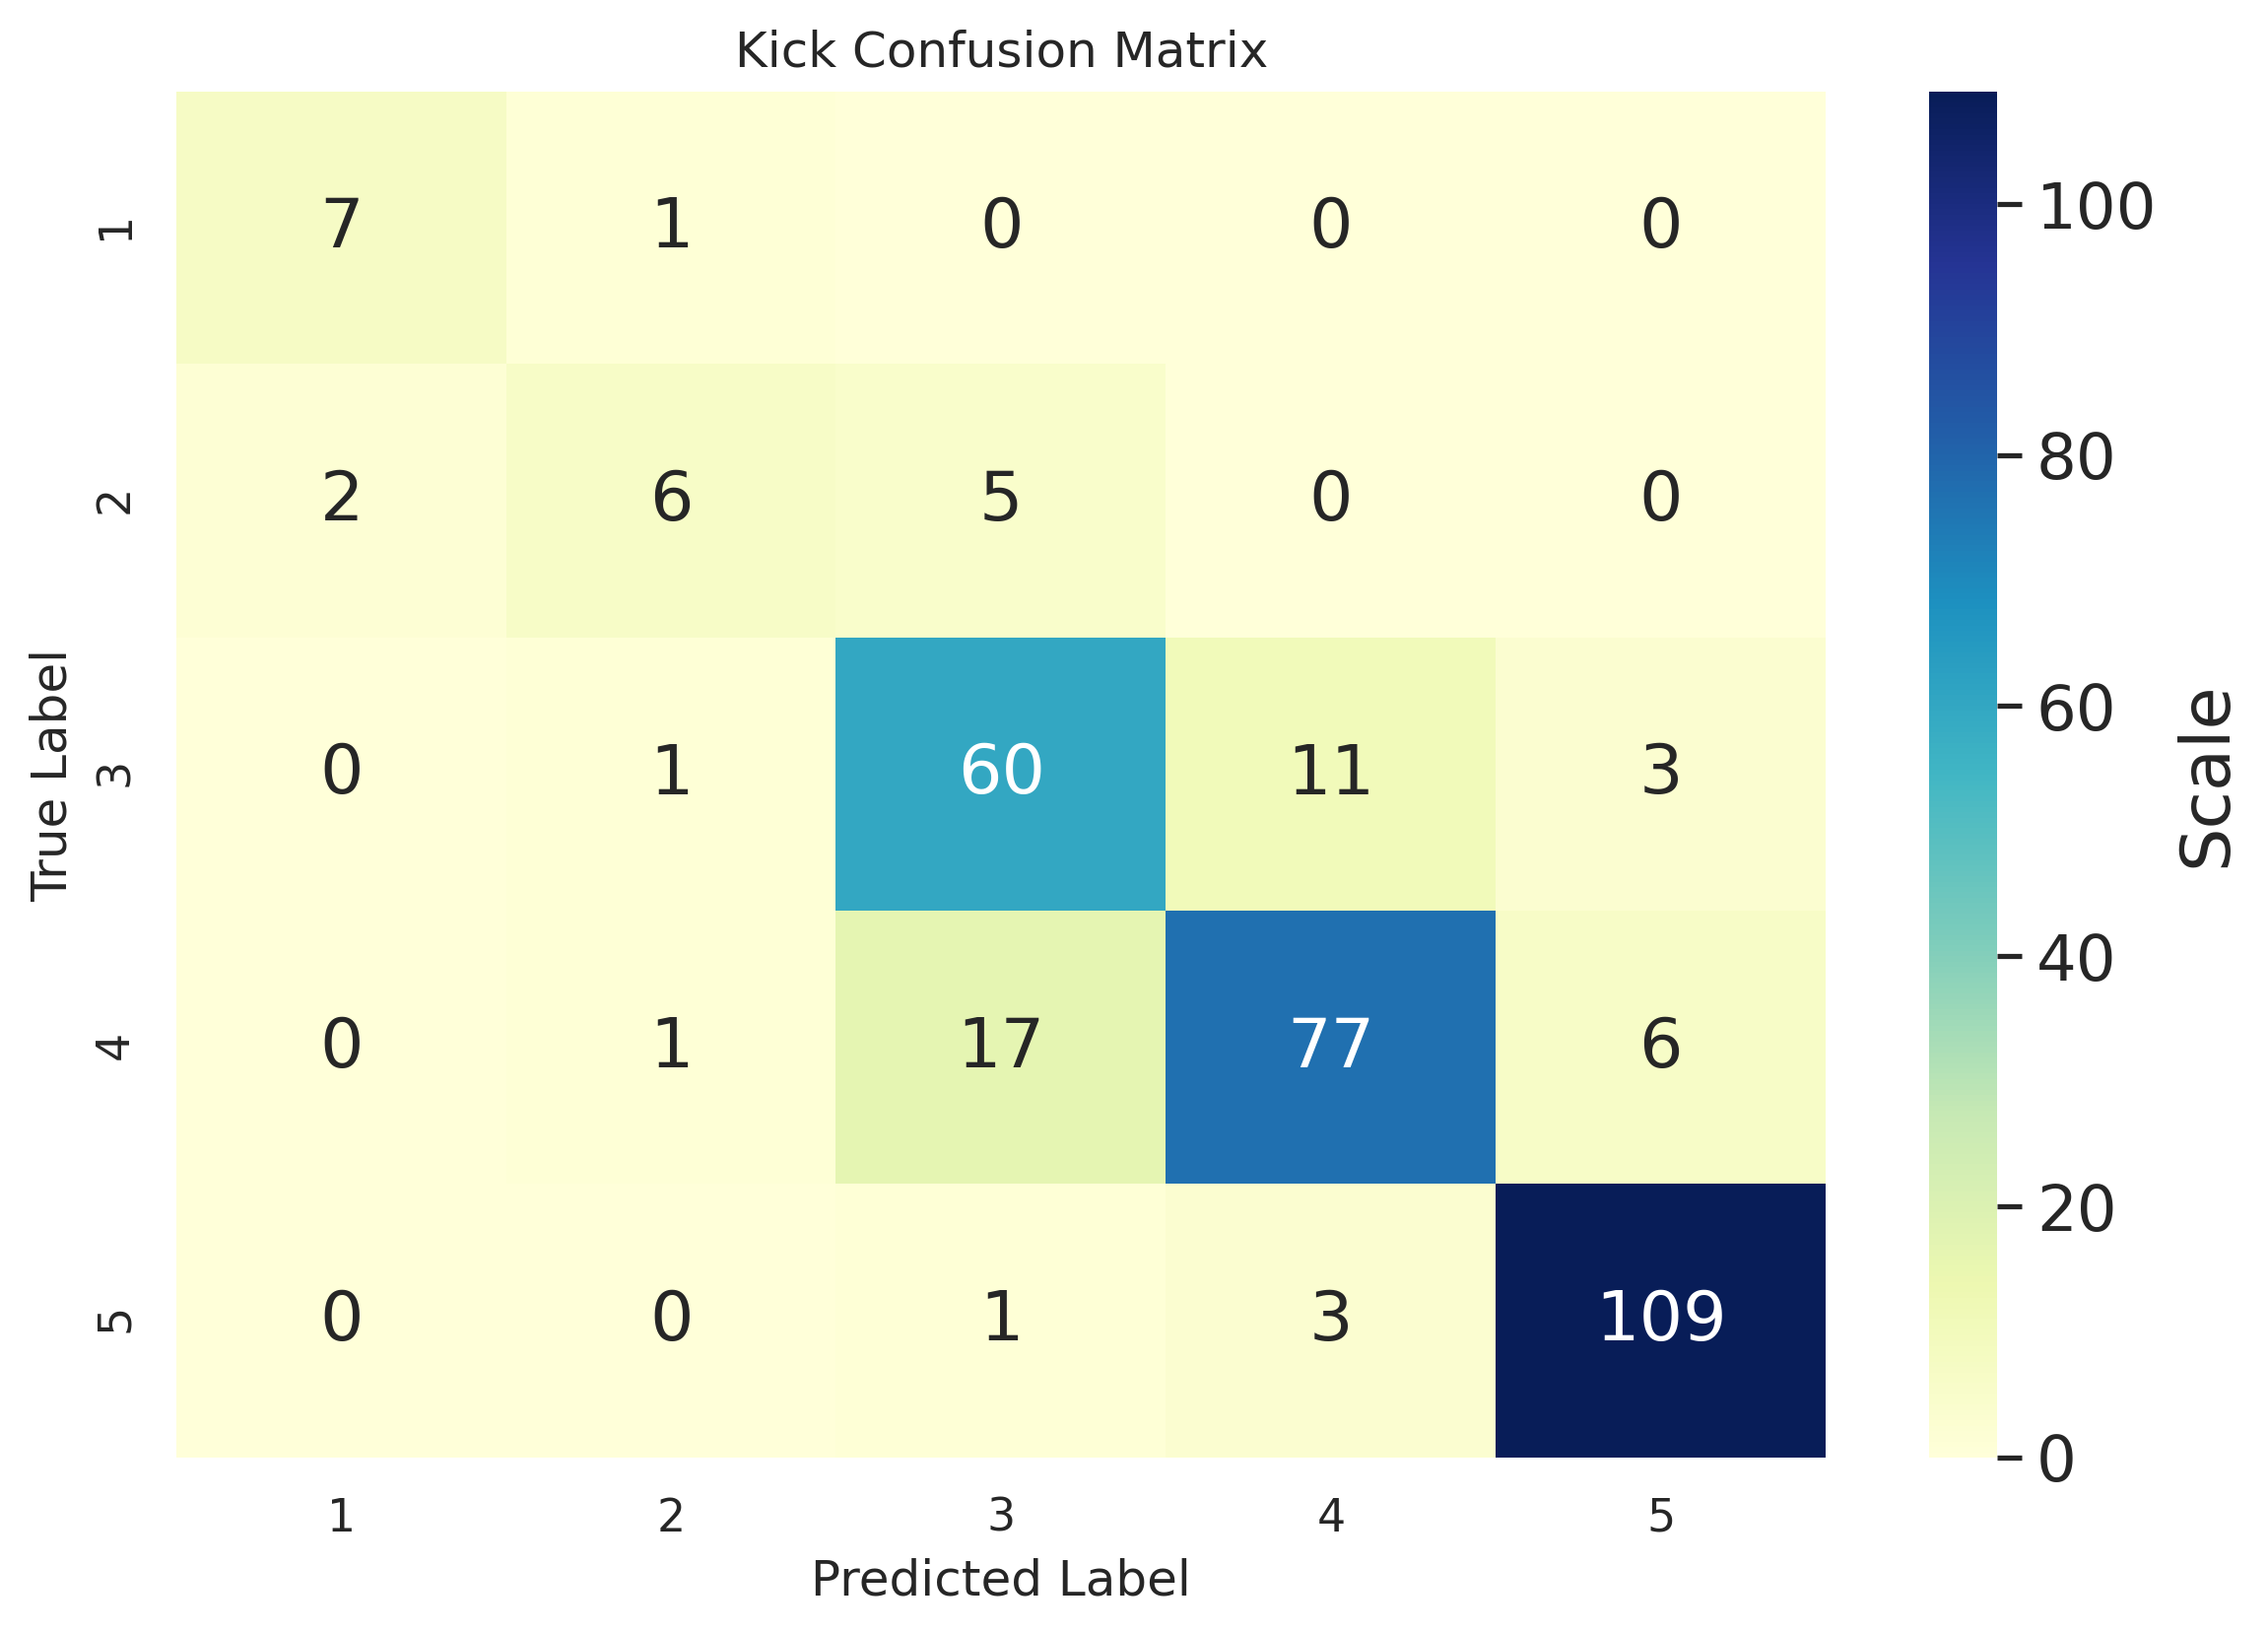
\includegraphics[width=\linewidth]{./immagini/second_classification/kick_cm.png}
		\caption{Matrice di confusione per la cassa}
		\label{fig:cm_2d}
	\end{subfigure}
	\caption{Matrici di confusione della prima fase}
	\label{fig:cm_2}
\end{figure}

%SPIEGA QUALI SONO I PARAMETRI  CHE INFLUENZANO I RISULTATI, GRANULARITÀ, WINDOW LENGTH E OVERLAP.
Questi risultati sono stati ottenuti effettuando una classificazione dove ogni sub campione è esattamente 8820 campioni, quindi 0.2s, per il campione successivo si esegue uno shift di 4410 campioni, ottenendo 0.1s di granularità e di overlap\footnote{Il tempo di sovrapponimento tra un sub-campione e l'altro}\\

Nei risultati ottenuti è possibile notare un peggioramento delle predizioni in modo particolare nel rullante, precisamente con un 51\% di istanze classificate correttamente per il rullante spazzolato e un 41\% per il colpo semplice di rullante. Con la cassa è stato ottenuto invece quello che è il risultato migiore con l'83\% di istanze classificate in modo corretto. Questa così ampia divergenza, così come per i risultati ottenuti precedentemente, è data dalla forma e dell'onda sonora in se. Infatti la cassa genera un onda con transiente molto marcato, e facilmente riconoscibile con le features utilizzate, che decade in modo molto rapido differentemente da quanto invece succede con il rullante, in particolar modo quello spazzolato. Un altro aspetto che influisce sull'abilità di riconoscere o meno un'onda sonora da un rumore è dato dall'intensità del segnale generato, infatti il rullante spazzolato genera un'onda con un ampiezza molto inferiore, difficilmente distinguibile da quello che è il rumore. L'ultimo aspetto ma non meno importante riguarda come sono stati selezionati i campioni per allenare la macchina, la numerosità dei campioni estratti e la qualità delle registrazioni utilizzate, tutti questi parametri possono influenzare pesantemente quelli che sono i risultati. Un numero maggiore di campioni potrebbe insegnare in modo migliore alla macchina la quale sarà in grado di costruire un albero di decisione migliore, come anche delle registrazioni migliori o con  volumi maggiori per alcuni strumenti dove possibile.